\section{Data Collection and Basic Analysis}
\label{sec:meth}

This section discusses how we collect data and metadata from VirusTotal
and how we preprocess them.
We also present the analysis results of their basic properties, 
before delving into more advanced analysis in later sections.


\begin{table}[h!]
\centering
\footnotesize
{
\begin{tabular}{l|l}
\hline
Metadata Field & Explanation \\
\hline                            
%\cline{1-1}
{\bf name}      & submitted file name \\
{\bf link}      & where to download the file \\
{\bf timestamp} & timestamp when the submission was made \\
{\bf source\_country} & the country where the submission was made \\
{\bf source\_id} & user ID who made the submission\\
{\bf size} & file size \\
{\bf type} & file type \\
{\bf tags} & labels with more specific information for each {\bf type}\\
{\bf first\_seen} & when the same file was first submitted \\
{\bf last\_seen} & when the same file was last submitted \\
{\bf hashes} & sha1, sha256, md5, and vhash\\
{\bf ssdeep} & ssdeep digest string \\
{\bf total} & number of engines analyzing the file \\
{\bf positives} & number of engines that flagged the file as malicious \\
{\bf positives\_delta} & changes in {\bf positives} across different submissions\\
{\bf report} & detailed detection report from each AV engine \\
\hline
\end{tabular}
}
\caption{VirusTotal Metadata. 
%\footnotesize{
(Fields for each submission retrieved from VirusTotal through distribution API and their related explanation.
One file could be submitted multiple times by different users.)
%}
}
\label{tab:fields}
\end{table}


\subsection{VirusTotal}
\yiying{we need to first introduce VT. what does it do, what does it provide, etc.}
\vt\ is a free online malware detection tool? etc.
It's used widely etc.
It's been around for ** years etc.
It's the only open access to real malwares?
Are users of VT mostly AV companies, software companies, OS companies, normal user, attackers? Do we have any way to tell or guess this?

\yiying{how do people use VT, how does VT use AV engines and generat its report}
For each \pe\ submission, \vt\ uses a set of anti-virus engines to analyze it.

\vt\ provides open APIs to access and download both the metadata of all submissions and detection results.
These APIs work like a pipe or a callback registering method.
After a user opens the API and establish ** to \vt, \vt\ will keep returning metadata for latest files submitted to the user.
blabla

\vt\ provides rich metadata
Table~\ref{tab:fields} shows the metadata fields and their meaning.  
The original submitted files from \vt\ can be downloaded using the {\bf link} field in the metadata.

\subsection{Data Collection and Preprocessing}
We collected \yiying{all?} metadata for all submissions to \vt\ from May 7th, 2016 to September 6th, 2016,
with a total of 151 million submissions. 
\yiying{We need some explanation here about why only four months of data is collected. maybe something like we found four months' data is already enough to make meaningful conclusions?}

We performed our data collection using \vt{}’s distribution API.
We insert all collected metadata into a table in Cassandra~\cite{Cassandra} 
using the combination of sha256, source\_id, and timestamp as the key. \yiying{fill the proper bib for cassandra}

\begin{figure}[t!]
\begin{center}
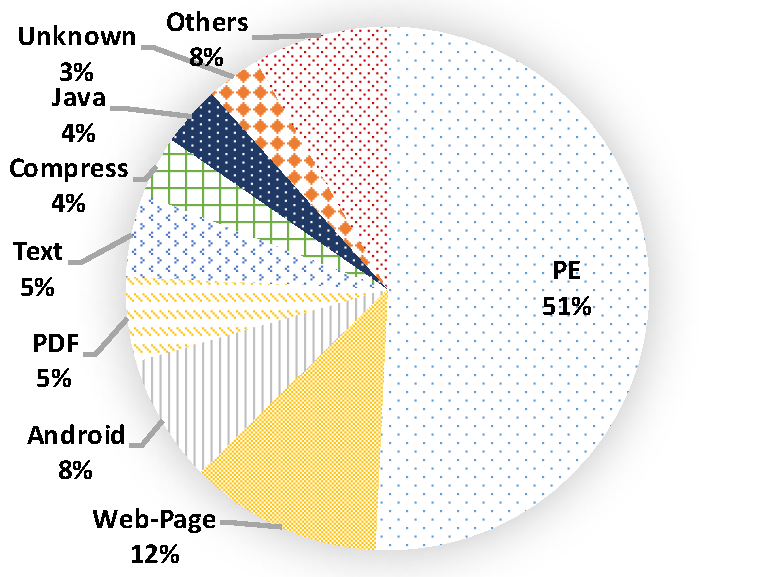
\includegraphics[width=2.in]{figure/type}
\caption{File type distributions.
%{\footnotesize{
(File types and their distributions for all VirusTotal submissions from 05/07/2016 to 09/06/2016.)
%}
}
\label{fig:type}
\end{center}
%\vspace{-0.25in}
\end{figure}


Figure~\ref{fig:type} shows the file type distribution for all submissions. 
Among all file types, Windows \textit{Portable Executable} ({\em \pe}) files, or ``Win32EXE'' and ``Win32DLL'' files, 
are the most frequently submitted type,
accounting for 51\% of all submissions.
%which conforms with a previous study~\cite{SongAPsys2016}.
Web pages and malwares on Android account for the second and third largest submissions, 
with 12\% and 8\% of all submissions respectively. 
Other popular file types include PDF, Text, compressed files, and Java files. 

Since PE files are the most common type,
we focus our study in this paper on \pe\ files 
and leave studies on other types of malwares for future. 
%If the type field for a submission is either ``Win32EXE'' or ``Win32DLL'', 
%we consider the submission is a PE file. 
In total, we collected 76 million \pe\ submissions.

\subsection{Basic Analysis}
After collecting data, we first conducted a set of basic analysis 
to learn the 



\begin{figure}[t!]
\begin{center}
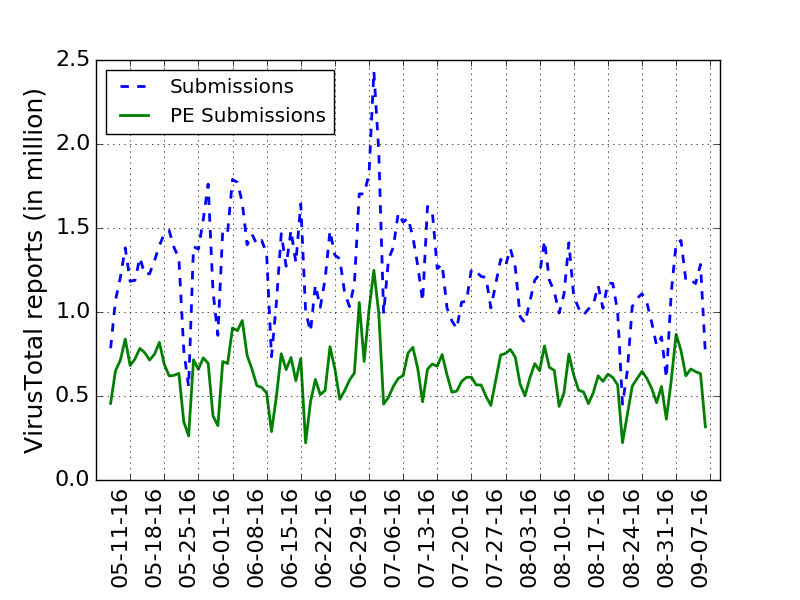
\includegraphics[width=2in]{figure/Submissions}
\caption{The number of files and PE files.
%{\footnotesize{
(The number of suspicious files and the number of PE files submitted to VirusTotal from 05/07/2016 to 09/06/2016.)
%}
}
\label{fig:subnum}
\end{center}
%\vspace{-0.25in}
\end{figure}

\begin{figure}[t!]
\begin{center}
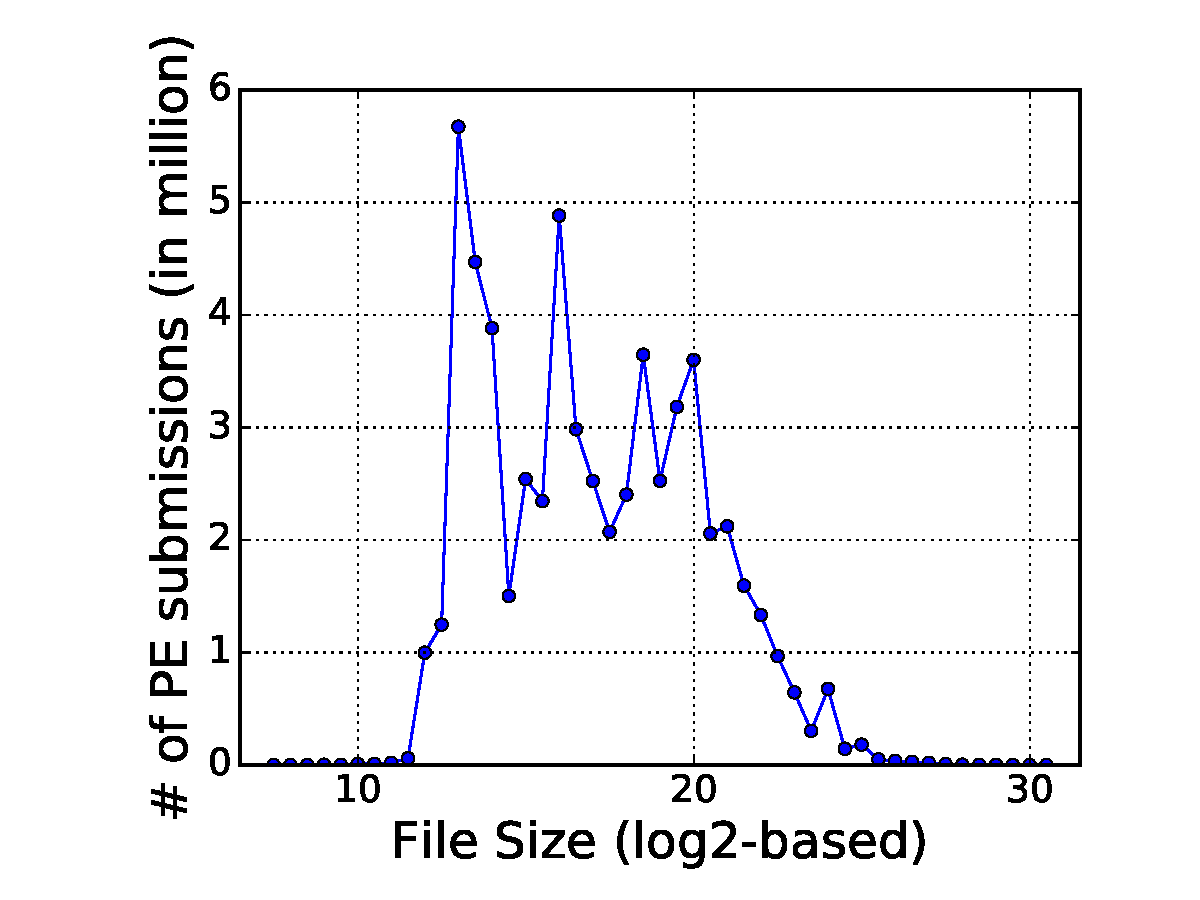
\includegraphics[width=2.5in]{figure/pesize}
\mycaption{fig:pesize}{File size distribution for PE submissions.}
{\footnotesize{(How file size distributes among all PE submissions we collect. 
Results from log2 are rounded up to nearest 0.5.)}}
\end{center}
%\vspace{-0.25in}
\end{figure}
\noindent{\bf Submission temporal, geo-location, and size distribution.} 
Figure~\ref{fig:subnum} plots the number of submissions of all types and the number of \pe\ submissions per day 
over the whole collection period.
There are a large amount of submissions every day
and the amount of submissions is fairly stable over the whole collection period.
The same conclusion can be made to \pe\ submissions.

\yiying{we still need the country distribution}

Figure~\ref{fig:pesize} shows the file size distribution for PE submissions. 
The smallest PE file is only xxx bytes, and the largest one is more than xxx\,MB. 
xxx\% of PE file fall into the range from xx\,KB to xx\,MB. 

\begin{figure}[t!]
\begin{center}
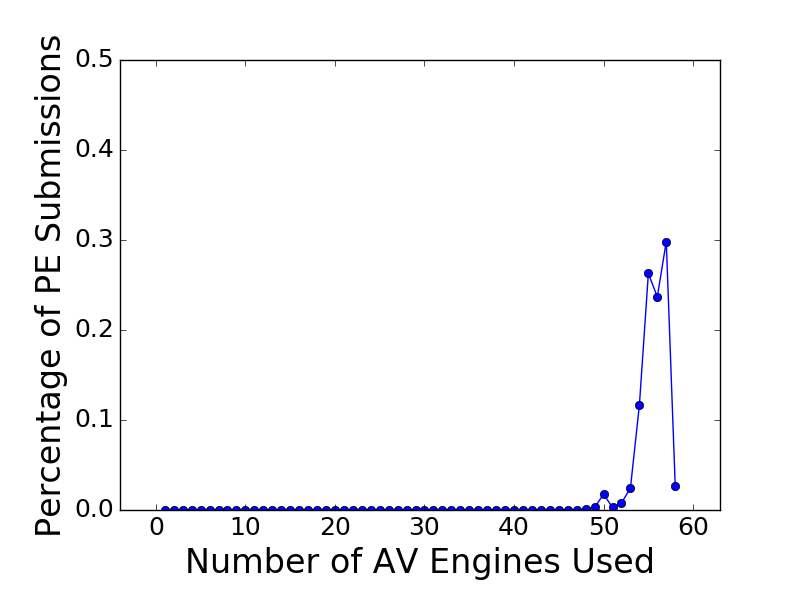
\includegraphics[width=2in]{figure/numVendor}
\caption{The distribution for the number of used anti-virus engines.
(How the number of applied anti-virus engines distributes among all PE submissions.
)
}
\label{fig:vendornum}

\end{center}
%\vspace{-0.25in}
\end{figure}
\begin{figure}[t!]
\begin{center}
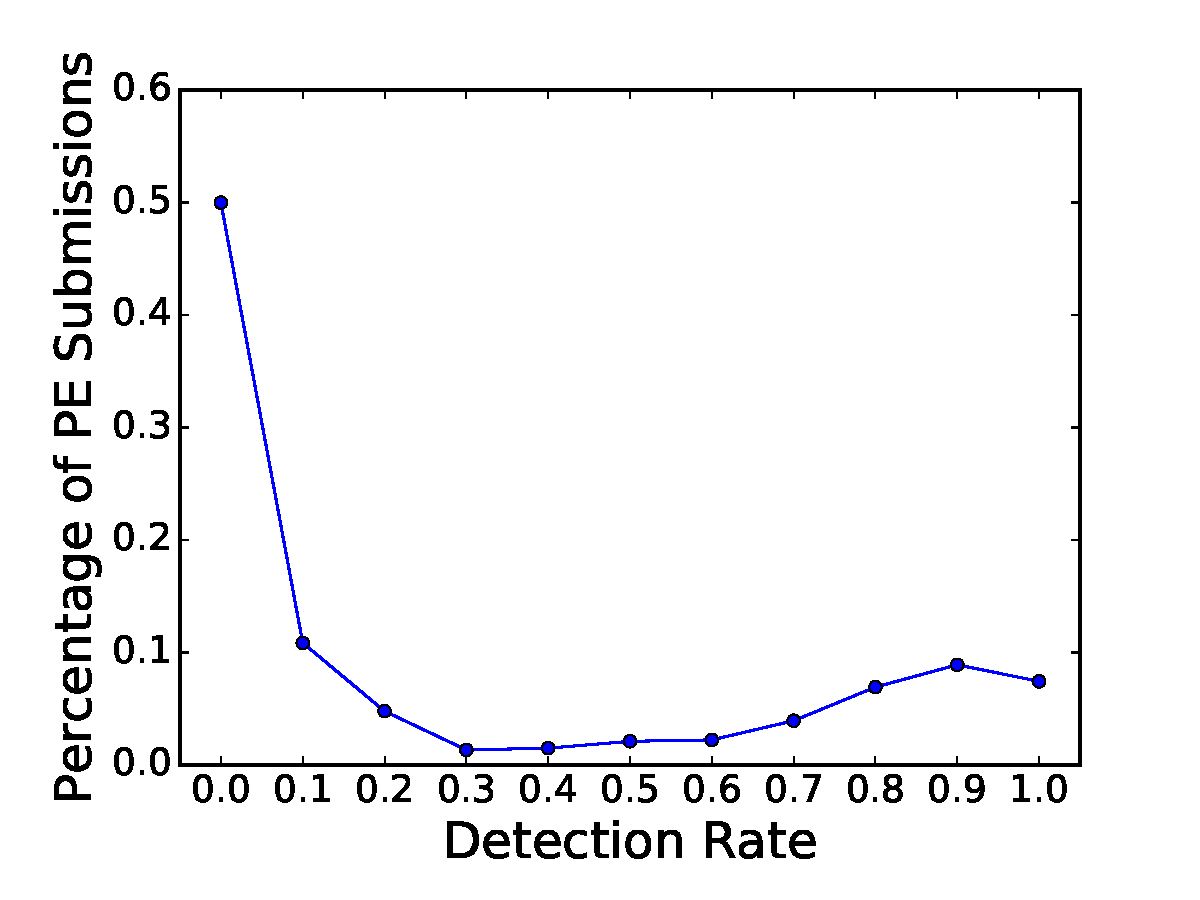
\includegraphics[width=2in]{figure/DetectionRate}
\caption{The distribution for detection rate.
(How detection rate distributes among all PE submissions. 
Each detection rate is rounded up to nearest 0.05.)
}
\label{fig:detectiorate}
\end{center}
%\vspace{-0.25in}
\end{figure}
\noindent{\textit{\underline{Anti-virus engines and detection basic analysis.}}}
%As shown in Table~\ref{tab:fields}, 
%total field is to represent the number of used anti-virus engines. 
Figure~\ref{fig:vendornum} shows the distribution for the number of used anti-virus engines. 
More than 99\% of PE submissions are analyzed by at least 50 anti-virus engines. 
Some anti-virus engines will label a submitted PE file as malware, 
while others will not. 
Positives field in Table~\ref{tab:fields} represents the number of anti-virus engines labeling the submission as malwares. 

$$ \textrm{\textit{Detection Rate}} = \dfrac{positives}{total + 1}$$

Detection rate represents the percentage of engines labeling the submission as malware. 
Adding one to total is to avoid dividing 0 exception, and more importantly, 
to give submissions labeled as malwares by more engines higher detection rate. 
For example, after adding one, submissions analyzed by 50 engines and detected by 50 engines will have a higher detection rate 
than submissions analyzed by 1 engine and detected by 1 engine. 
This formula shares the same intuition from previous work~\cite{GuoICSE2010}, when computing reputations for bug reporters. 
A larger detection rate usually indicates a more malicious malware suggested by analyzed anti-virus engines. 
Figure~\ref{fig:detectiorate} shows how detection rate distributes among all PE submissions. 

One PE file could be submitted more than once to VirusTotal. 
There are 6.72\% PE files submitted more than once to VirusTotal. 
On average, each PE file is submitted 1.19 times. 
Some anti-virus engines may produce different detection results when analyzing the same file for different submissions.
We assume there is influence among different anti-virus vendors, 
and this influence is a very important reason causing engines to change their results.
We will discuss how we model this influence and how to predict possible detection result change by using our model in Section~\ref{sec:influ}.

\subsection{}
\yiying{I don't know what to call this paragraph. But it should go into a subsection}

Like all other empirical study works, 
our findings and conclusions need to be considered with our methodology in mind. 
We use distribution API to download submissions' metadata from VirusTotal. 
There is no guarantee that all data can be successfully downloaded. 
It could be possible that some files are submitted to VirusTotal, 
but we fail to get their information from VirusTotal.
Although we have collected huge amount of malware information from VirusTotal,
we do believe that there are malwares never submitted to VirusTotal, 
or submitted to VirusTotal much later than they appear in the real world. 
However, there are no conceivable ways to study them.
We believe the 4-month malware information we collect can serve as a representative sample for malwares in the real world. 
